%% %%%%%%%%%%%%%%%%%%%%%%%%%%%%%%%%%%%%%%%%%%%%%%%%%
%% Template for a conference paper, prepared for the
%% Food and Resource Economics Department - IFAS
%% UNIVERSITY OF FLORIDA
%% %%%%%%%%%%%%%%%%%%%%%%%%%%%%%%%%%%%%%%%%%%%%%%%%%
%% Version 1.0 // November 2019
%% %%%%%%%%%%%%%%%%%%%%%%%%%%%%%%%%%%%%%%%%%%%%%%%%%
%% Ariel Soto-Caro
%%  - asotocaro@ufl.edu
%%  - arielsotocaro@gmail.com
%% %%%%%%%%%%%%%%%%%%%%%%%%%%%%%%%%%%%%%%%%%%%%%%%%%
\documentclass[11pt]{article}
\usepackage{UF_FRED_paper_style}
\usepackage{tabularx} 
\usepackage{lipsum}  %% Package to create dummy text (comment or erase before start)
\usepackage{multirow}
\usepackage[normalem]{ulem}

\usepackage{tabularx} % in the preamble
\usepackage{todonotes}
% ....

\useunder{\uline}{\ul}{}
%% ===============================================
%% Setting the line spacing (3 options: only pick one)
% \doublespacing
% \singlespacing
\onehalfspacing
%% ===============================================

\setlength{\droptitle}{-5em} %% Don't touch

% %%%%%%%%%%%%%%%%%%%%%%%%%%%%%%%%%%%%%%%%%%%%%%%%%%%%%%%%%%
% SET THE TITLE
% %%%%%%%%%%%%%%%%%%%%%%%%%%%%%%%%%%%%%%%%%%%%%%%%%%%%%%%%%%

% TITLE:
\title{Measures of quality for Dialogue Utterance Generation (working title)
}

% AUTHORS:
\author{Marco Moresi\\% Name author
    \href{mailto:moresi@hhu.de}{\texttt{moresi@hhu.de}} %% Email author 1 
%\and Forth Author\\% Name author
%    \href{mailto:forthuthor@ufl.edu}{\texttt{forthuthor@ufl.edu}}%% Email author 4
    }
    
% DATE:
\date{\today}

% %%%%%%%%%%%%%%%%%%%%%%%%%%%%%%%%%%%%%%%%%%%%%%%%%%%%%%%%%%
% %%%%%%%%%%%%%%%%%%%%%%%%%%%%%%%%%%%%%%%%%%%%%%%%%%%%%%%%%%
\begin{document}
% %%%%%%%%%%%%%%%%%%%%%%%%%%%%%%%%%%%%%%%%%%%%%%%%%%%%%%%%%%
% %%%%%%%%%%%%%%%%%%%%%%%%%%%%%%%%%%%%%%%%%%%%%%%%%%%%%%%%%%
% ABSTRACT
% %%%%%%%%%%%%%%%%%%%%%%%%%%%%%%%%%%%%%%%%%%%%%%%%%%%%%%%%%%
% %%%%%%%%%%%%%%%%%%%%%%%%%%%%%%%%%%%%%%%%%%%%%%%%%%%%%%%%%%
{\setstretch{.8}
\maketitle
% %%%%%%%%%%%%%%%%%%
\begin{abstract}
% CONTENT OF ABS HERE--------------------------------------
Natural language generation (NLG) is a crucial component of task-oriented dialog systems and it has a significant impact both on usability and perceived quality. The NLG module converts a dialog act represented in a semantic form into a response in natural language. Typically these systems are evaluated by examining whether the system realizes all concepts from the semantic form,  measured by \emph{slot error rate}, and compares a model's generated response to a single target response using automated measures from machine translation such as BLEU, ROUGE, and METEOR.

In this work, we investigate the impact of cases when the system realizes a concept that does not appear in the semantic form.

We also propose to replace the automatic measures such as BLEU with a transformed discriminator that is trained to distinguish between the human utterance and an utterance generated by a language model.

We believe that these measures give a much better insight into capabilities of the NLG component than previously considered.


%MM: add what we want to talk here

% END CONTENT ABS------------------------------------------
\noindent
\textit{\textbf{Keywords: }%
Natural Language Generation; Oriented task dialogue system; Evaluation Metrics.} \\ %% <-- Keywords HERE!

\end{abstract}
}

% %%%%%%%%%%%%%%%%%%%%%%%%%%%%%%%%%%%%%%%%%%%%%%%%%%%%%%%%%%
% %%%%%%%%%%%%%%%%%%%%%%%%%%%%%%%%%%%%%%%%%%%%%%%%%%%%%%%%%%
% BODY OF THE DOCUMENT
% %%%%%%%%%%%%%%%%%%%%%%%%%%%%%%%%%%%%%%%%%%%%%%%%%%%%%%%%%%
% %%%%%%%%%%%%%%%%%%%%%%%%%%%%%%%%%%%%%%%%%%%%%%%%%%%%%%%%%%

\section{Introduction}

In recent years, task-oriented dialogue systems have gained acceptance and popularity, as evident from the surge of personal assistants. In a typical task-oriented dialog system, the user can perform actions such as, booking a hotel, restaurant reservation, or buying a train ticket. In these systems, the Natural Language Generation (NLG) module plays a crucial role as it  converts the system action (e.g, often represented in a semantic form given by the dialogue policy) into a final utterance in natural language. Therefore, the generated sentence should adequately represent the semantic meaning while retaining fluency, as described on ~\cite{stent2005} to catch the user's attention. What makes the NLG module so critical, is that it is the last module in the pipeline of a dialogue system meaning that its output directly influences the user experience. Nowadays, despite all the efforts made by the community, automatically evaluating the quality of the NLG  models remains an open question.

Automatic measures are widely used acorss natural language processing (NLP) tasks, for example, BLEU ~\cite{Papineni2002} and METEOR ~\cite{banerjee2005} for machine translation models, and ROUGE ~\cite{lin-2004-rouge} for summarization. These metrics are also used by dialogue researchers ~\cite{ritter2011data, Witteveen_2019, cai2020learning, wen-etal-2017-network, wen2015semantically}. However, these metrics assume that a correct generated utterance has significant word overlap with the ground truth response. In metrics for dialogue systems this is a strong assumption because there is a significant diversity in the space of valid replies given a semantic representation. A significant drawback of these metrics is also that they only considering the words without their underlying meaning, so polysemity of words is not considered. 

In this report we investigate the impact of cases when the system realizes a concept that does not appear in the semantic form.  

We also propose to replace the automatic measures such as BLEU with a transformer discriminator that is trained to distinguish between the human utterance and an utterance generated by variety of language models.

We demonstrate that these measures give a much better insight into capabilities of the NLG component than previously considered.

\section{Background}

\begin{figure}%
    \centering
    \subfloat[Task-oriented dialogue system architecture]{{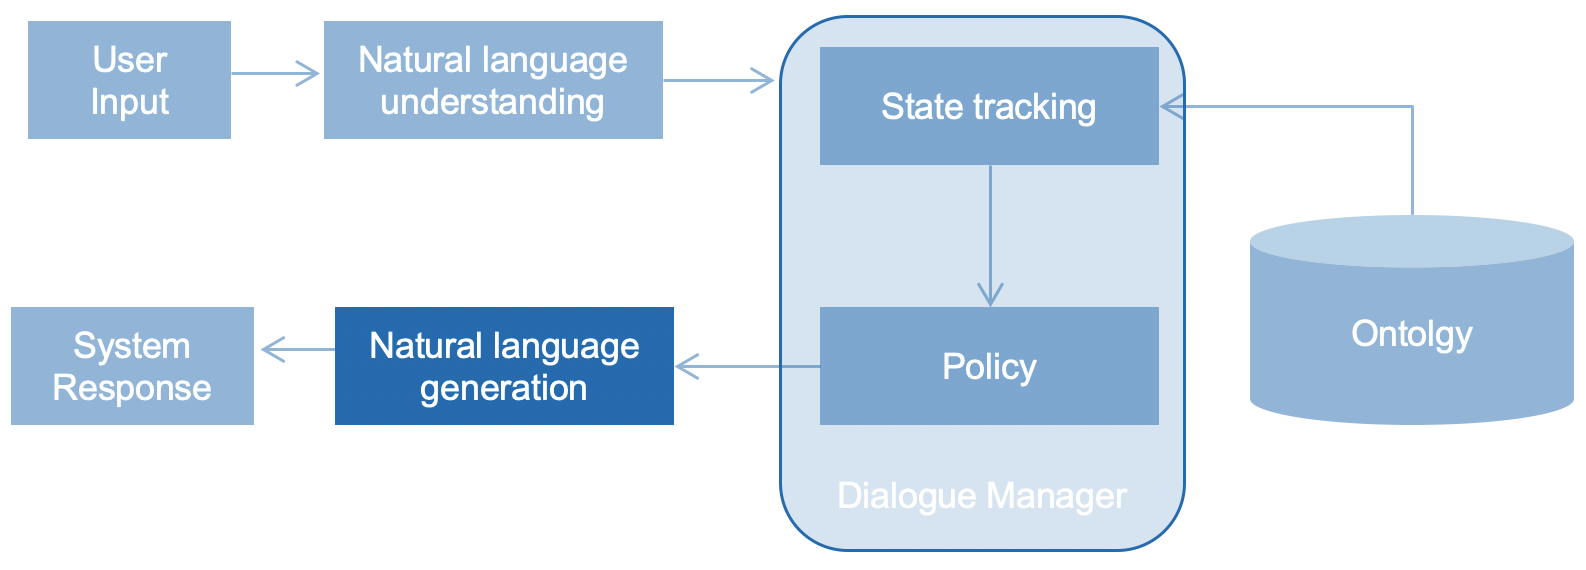
\includegraphics[width=10cm]{figures/dialogue.png} }}%
    \qquad
    \subfloat[Dialogue Act]{{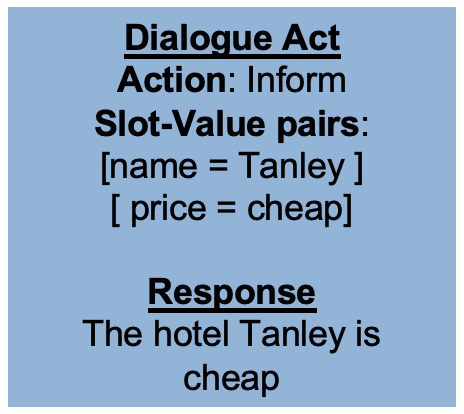
\includegraphics[width=4cm]{figures/dialogue_act.png} }}%
    \caption{The NLG module in the overall task-oriented dialog system. (a) The NLG module is in dark blue in the diagram. (b) Example of dialogue act, including action and slot-value pairs and its corresponding response}%
    \label{fig:dialogue}%
\end{figure}

%Add more cites for each module of the pipeline
A typical task-oriented spoken dialog system uses a pipeline architecture, as shown in Figure~\ref{fig:dialogue}(a). Firstly, the user input is interpreted by the Natural Language Understanding module extracting the relevant information from the user. Then this information is passed to the Dialogue manager which consists of two sub-modules, State Tracking and Policy. The State Tracking~\cite{heck2020trippy} is in charge of maintaining the state of the dialogue along with all the conversation. The output of the State Tracking is passed to the Policy module, which produces a dialogue act based on the knowledge provided by the Ontology. The Ontology is the underlying database or a knowledge-base that contains the entities that the system can talk about. These entities are further described with semantic concepts, such as domain, slot and value. Lastly, the dialogue act (DA) generated by the Policy is feed into the NLG which converts it into a system utterance in natural language.
In particular, a DA is a concatenation of an Action (ACT) and a set of slot-value pairs
 $(s_{1},v_{1}), .. , (s_{n},v_{n})$. 

$$ DA = [ACT{(s_{1},v_{1}), ... ,(s_{n},v_{n})}] $$

In this paper, the objective is to understand better how to evaluate this last module.


\subsection{Language models as generators} \label{language_model}
Language Models are probably one of the most popular mechanisms to generate natural language. Language modeling is the development of probabilistic models that are able to predict the next word in the sequence given the words that precede it.
A language model learns the probability of word occurrence based on examples of text. Simpler models may look at a context of a short sequence of words, whereas larger models may work at the level of sentences or paragraphs. Most commonly, language models operate at the level of words.

The Long Short Term Memory (LSTM)~\cite{hochreiter1997long} network, has been shown that it is very effective for a wide range of different tasks such as Language Generation, Language classification among others. It is able to capture long term dependencies that a Recurrent Neural Network can not do because of the vanishing gradient problem~\cite{bengio1994learning}. In language model task learning long term dependencies is something crucial to achieving a good quality of the generated text.

Recently, the self-attention-based Transformer model achieved state-of-the-art performance on various NLP task~\cite{vaswani2017attention}. The Transformer architecture replaces the RNN cells with self-attention and fully connected layers. Together with positional embeddings, Transformers are able to capture long-term dependencies.

GPT-2~\cite{radford2019language} is probably one of the most popular language model nowadays, it uses a variant of the Transformer  architecture~\cite{vaswani2017attention}. It is an auto-regressive language model that leverages 12-24 layers of masked, multi-head self-attention Transformers. GPT-2 is pre-trained on massive text data that consists of 8 million web pages a total of 40Gb of text data. It has superior performance in characterizing human language data distribution and knowledge transfer. Given text prompts, GPT-2 can generate realistic sentences.

\todo{MG: Can you say what is the main difference between BERT and GPT-2?}

\todo{MM: I explain the delexicalization in section \ref{new_slot_error} Shall I move it after this section. I wanted to explain the delexicalization in the context of the metric that we propose and explain why we need a semantic dictionary}
\subsection{Semantically-conditioned language models as dialogue generators}\label{conditioned-generators}
Within the context of task-oriented dialogue, we need a way to control the natural language generator models, to make sure that the intended information is passed to the user. In this report we examine three such generators.

\textbf{Semantically Conditioned LSTM (SC-LSTM)} by Wen et.al~\cite{wen-etal-2015-semantically},  is based on adding a new control mechanism to a LSTM ~\cite{hochreiter1997long} network in order to control that all the pair slot-values present in the dialogue are present in the generated sentence.

\textbf{Semantically Conditioned Dialog Response Generation (HDSA)} by Chen et. al~\cite{chen2019semantically},  is based on a  hierarchical disentangled self-attention network, which allows to model different domain and control the slot-values that it generates. It encodes the dialogue act into a tree representation and uses it to create the connections between the heads in the attention layers, thus using the training data efficiently.

\textbf{Semantically Conditioned GPT (SC-GPT)} by Peng et. al.~\cite{peng2020fewshot} is based on the pre-trained  GPT-2~\cite{radford2019language} model, leveraging all the information learned during the pre-training. In order to condition the generation, the dialogue act along with the pairs slot-values are utilized as context (prompt) of GPT-2. The promt is concatenated to the target sentence during training and therefore the model learns the expected output given a prompt. During generation, it is only necessary to feed the prompt into the model.


\subsection{Transformer as a discriminator}\label{discriminator}

In addition to using transformers as generators, it is common to use them as encoders for discriminative tasks. BERT~\cite{devlin2018bert} is particularly useful in this respect. It uses a variant of the Transformer  architecture~\cite{vaswani2017attention} and is trained on massive corpora, Books Corpus (800M words), and English Wikipedia (2,500M words), and allows fast fine-tuning to allow a wide range of practical applications. BERT generates contextual embeddings, meaning that it can generate different vector representations for the same word in different sentences depending on the surrounding words. In addition, as BERT can capture information about the relation between tokens in the sequence. This is why, it performs well in the classification tasks.



\subsection{Commonly considered metrics for NLG} \label{slot_error}
During the evaluation in task-oriented dialogue, it is on one hand important to examine whether the system realised all the concepts from the dialogue act and on the other hand how similar that relasation is to human provided target. 

In ~\cite{wen-etal-2015-semantically} the metric slot error rate is defined as  
$$
\mathrm{ERR}=\frac{p+q}{N},
$$
where $N$ is the total number of slots in the DA, $p$ is the number of missing slot and $q$ is the number of redundant slots. This metric is calculated utilizing the delexicalized version of the utterance.

As defined above, this metric does not consider the cases when the slot value pairs that a model generates were not in the original DA. Introducing unnecessary information in the utterance that can drive to a confusion of the user during the utilization of the system is therefore not captured.


\section{Improved automatic measures for NLG}
% select a "different" name for the metric
\subsection{Slot Error with extras} \label{new_slot_error}
Here we modify the slot error rate to consider the slot-value pairs that are not present in the original DA, called \emph{extras},

$$\mathrm{ERR+extras}=\frac{p+q+e}{N}.$$

Considering that SC-LSTM and HDSA models generate the utterances delexicalized so no post-process is necessary. However, SC-GPT generates natural language directly, so we need to delexicalise it to extract information about $p$, $q$, $e$ and $N$.  We implement a post-process stage where we use the corresponding dialogue act from the test set for each utterance that SC-GPT generates. Using the dialogue act we replace the values that appear in it and in the generated sentence for special tokens that are agnostic of the slot value. After this, we build a semantic dictionary with all the slot-value pairs available in MultiWoz~\cite{budzianowski-etal-2018-multiwoz} dataset and we use this to find the extra values generated in the sentence. An example of this post-process procedure is shown in the Table~\ref{tab:delexicalization} where it can be seen that using only the dialogue act is not enough to find the realizations of extra slots.

\todo{MG: This was not a good example as location was already part of DA, I removed it from DA}
\begin{table}[H]
\centering
\begin{tabularx}{\textwidth}{l|X}
\textbf{Dialogue Act (DA)} & Inform(hotel\_name=Tanley, pricerange=cheap) \\ \hline
\textbf{Generated Sentence} & The hotel Tanley is cheap and it is located in the west \\ \hline
\textbf{\begin{tabular}[c]{@{}l@{}}Delexicalized Sentence\\ with DA\end{tabular}} & The hotel {[}hotel\_name{]} is {[}pricerange{]} and it is located in the west \\ \hline
\textbf{\begin{tabular}[c]{@{}l@{}}Delexicalized Sentence\\ with DA and Semantic \\ Dictionary\end{tabular}} & The hotel {[}hotel\_name{]} is {[}pricerange{]} and it is located in the {[}location{]}
\end{tabularx}
\caption{Delexicalization process, utilizing the corresponding dialogue act and the semantic dictionary to find extra slot values}
\label{tab:delexicalization}
\end{table}


%We test this new metric in two models that belong to the state-of-the-art in NLG for dialogue Systems, SC-GPT by Peng et. al.~\cite{peng2020fewshot} and HDSA by Chen et. al~\cite{chen2019semantically}. Also, we tested it in one of the most relevant models in the area Semantically conditioned LSTM by Wen et.al~\cite{wen-etal-2015-semantically}.



\subsection{BERT as a Discriminator of Generated Utterances}
% Description of the methods here
Instead of relying on measures such as BLUE and METEOR which directly do n-gram matching, we propose to train a BERT discriminator which distinguishes between human response and a language model generated response. Note that at this point we do not consider semantically conditioned language modelling response as we believe that the issue of realising semantics should be addressed with slot error rate.

\subsubsection{Training data}\label{sec:dataset}
The aim is to produce a training set for a discriminator consisting of human utterances (positive examples) and utterances generated by a language model (negative examples). The score that the discriminator gives is inversely related to the measure of quality. To do that we build three different language models to generate the negative examples, a language model using a LSTM~\cite{hochreiter1997long} architecture, another using Transformer~\cite{vaswani2017attention} encoder layers and the last one using GPT-2~\cite{radford2019language}.

All models are trained as language models, using all the system utterances that belong to dialogues in MultiWoz 2.0 (56778 responses in total) for training. The models are trained until they converge. After this,  each of the three trained language models, separately generates  on third of negative samples as the Multiwoz split: 56778, 7374, 7372 sentences for train, validation, and test set respectively. In that way we end up with a balanced dataset for training a discriminator.


In Table~\ref{tab:dataset} can be seen the original size of the split and the augmented versions with all the different proposed models.

\begin{table}[H]
\centering
\begin{tabular}{c|c|c|c}
\multicolumn{1}{l|}{\textbf{}} & \textbf{Train} & \textbf{Valid} & \textbf{Test} \\ \cline{2-4} 
\textbf{MultiWoz (MW)} & 56778 & 7374 & 7372 \\ \hline
%\textbf{\begin{tabular}[c]{@{}c@{}}Augmented MW\\ (LSTM LM)\end{tabular}} & 113556 & 14748 & 14744 \\ \hline
%\textbf{\begin{tabular}[c]{@{}c@{}}Augmented MW\\ (Transformer LM)\end{tabular}} & 113556 & 14748 & 14744 \\ \hline
%\textbf{\begin{tabular}[c]{@{}c@{}}Augmented MW\\ (GPT-2 LM)\end{tabular}} & 113556 & 14748 & 14744 \\ \hline
\textbf{\begin{tabular}[c]{@{}c@{}}Augmented MW\\ (LSTM + Transformer + GPT-2)\end{tabular}} & 113556 & 14748 & 14744 \\ \hline
\end{tabular}
\caption{Original Multiwoz dataset and the augmented version for binary classification using the Language models (LSTM, Transformer-based, GPT-2).}
\label{tab:dataset}
\end{table}


\subsection{The discriminator}
In Section\ref{discriminator} we presented BERT as the model that plays the role of the discriminator in this work. Using the BERT implementation of HugginFace~\cite{Wolf2019HuggingFacesTS} we create one discriminator model for the augmented dataset that we created Table~\ref{tab:dataset}. The Bert model is fine-tuned for sequence classification as a downstream task during 5 epochs.

In order to measure how good is BERT to distinguish the generated sentences with a language model from the human, we utilize the F1 score, which is a harmonic average between precision and recall. We calculate it for each label (positive and negative) and then we calculate the weighted average of the F1 values for each label, where the weights are the number of examples in each class.

Then the BERT discriminator model trained with augmented MultiWoz dataset LSTM, Transformer and GPT-2 we test the sentences generated by SC-LSTM, HDSA, and SC-GPT respectively.


\section{Experiments} %(WIP, revision is needed)
This section shows the different experiments conducted in order to evaluate and compare three models of NLG. Firstly in the subsection~\ref{results-new-slot-error} we present the results for the extension proposed for the Slot error metric. In Section~\ref{results-language-model} we present the results of the experiments using BERT as the discriminator between human utterances and generated by language models.

\subsection{New slot error}\label{results-new-slot-error}
In order to have a fair comparison we trained the models using MultiWoz2.0 dataset~\cite{budzianowski-etal-2018-multiwoz} following the original split. 

We evaluate each system with the new proposed metric on the test set, the results are shown in the Table~\ref{tab:err}
\begin{center}
\begin{table}[h]
\centering
\begin{tabular}{l|c|c|c|c|c}
 & Missing & Extra & Redundant & Slots\dagger & Error rate \\ \hline
SC-LSTM & 1535 & 599 & 347 & 10634  & 23.33 \\ \hline
HDSA & 688 & 589 & 20 & 10634  & 12.19 \\ \hline
SC-GPT* & 103 & 150 & 81 & 10634 & 3.14 \\ \hline

\end{tabular}
\caption{Error rate for each model evaluated on Multiwoz test set.  $\dagger$ number of ground truth slot. * a postprocess with a semantic dictionary was implemented.}
\label{tab:err}
\end{table}
\end{center}

Our improved measure shows some interesting behavior. HDSA outperforms SC-LSTM on missing and redundant slots, however, it has an equally high number of extras. SC-GPT on the other hand outperforms both models on missing and extra but not on redundant slots.

%Also, in Table~\ref{tab:err} can be seen that the Error rate in SC-GPT decreased in comparison with the other models but the number of extras slots still being a problem and it could generate confusion to the user because the model is given more information that it should give.

We also evaluate the models using the F1 score. The results are shown in Table~\ref{tab:f1}, but the deficiency  of HDSA and SC-GPT presented above is not as apparent. We therefore argue that it is important to utilise the improve slot error rate measure, as it dissects the capability of NLG to realise semantics.


\begin{center}
\begin{table}[H]
\centering
\begin{tabular}{l|c|c|c|c}
 & TP & FP & FN & F1 \\ \hline
 SC-LSTM & 8485 & 946 & 1535 &  0.872 \\ \hline
HDSA & 9946 & 609 & 668 &  0.938 \\ \hline
SC-GPT* & 10531 & 231 & 103 & 0.978\\ \hline
\end{tabular}
\caption{Entity F1 for each model evaluated on Multiwoz test set. * with post-processing utilising a semantic dictionary}
\label{tab:f1}
\end{table}
\end{center}

It can be seen in both, Table~\ref{tab:err} and Table~\ref{tab:f1}, SC-LSTM is the model that has a higher error rate and lowest F1 score while SC-GPT is the one with the lowest Error Rate and highest F1 as previously reported by~\cite{TODO}.\todo{CITE:}

\subsection{Discriminate utterances}\label{results-language-model}
\subsubsection{LSTM}
Table~\ref{tab:discriminator-results} shows the results of BERT as a discriminator on the validation set of the augmented dataset. The first four rows show the results on the portion of the dataset generated by each language model as well as the total performance Section~\ref{sec:dataset}. 

\begin{table}[h]
\centering
\begin{tabular}{|l|c|c|c|}
\hline
\multicolumn{1}{|c|}{\textbf{Discriminator}} & \multicolumn{1}{c|}{\textbf{\begin{tabular}[c]{@{}c@{}}Human Utterances\\ F1\end{tabular}}} & \multicolumn{1}{c|}{\textbf{\begin{tabular}[c]{@{}c@{}}Language Model\\ Utterances F1\end{tabular}}} & \multicolumn{1}{c|}{\textbf{\begin{tabular}[c]{@{}c@{}}Weighted Average\\ F1\end{tabular}}} \\ \hline
LSTM  & 0.7964 & 0.8254 & 0.8109 \\ \hline
Transformer  & 0.9814 & 0.9808 & 0.9811 \\ \hline
GPT-2  & 0.9055 & 0.8898 & 0.8977 \\ \hline
Combined\dagger & 0.9789 & 0.9789 & 0.9789 \\ \hline
\end{tabular}
\caption{Results of experiments using BERT as a discriminator between human utterances from dataset and the language model generated. Combined$\dagger$ discriminator is trained with dataset build with sentences from the three language models, LSTM, Transformer and GPT-2}
\label{tab:discriminator-results}
\end{table}


% This table shows the results of the combined discriminator testing the utterances from the language models. The results are confusing me.
%\begin{table}[]
%\begin{tabular}{|l|c|c|c|}
%\hline
%\textbf{Data} & \textbf{\begin{tabular}[c]{@{}c@{}}Human Utterances\\ F1\end{tabular}} & \textbf{\begin{tabular}[c]{@{}c@{}}Language Model\\ Utterances F1\end{tabular}} & \textbf{\begin{tabular}[c]{@{}c@{}}Weighted Average\\ F1\end{tabular}} \\ \hline
%LSTM & 0.6763 & 0.1301 & 0.4032 \\ \hline
%Transformer & 0.9737 & 0.9731 & 0.9734 \\ \hline
%GPT-2 & 0.7301 & 0.4391 & 0.5846 \\ \hline
%\end{tabular}
%\caption{}
%\label{tab:my-table}
%\end{table}


Using the Combined discriminator we test how good is the quality of the sentences generated by the models, SC-LSTM, HDSA, and SC-GPT. Table~\ref{tab:sem-conditioned} shows the results.


\begin{table}[H]
\centering
\begin{tabular}{|l|c|}
\hline
\multicolumn{1}{|c|}{\textbf{Data}} & \textbf{\begin{tabular}[c]{@{}c@{}}Sem. Conditioned\\ Utterances F1\end{tabular}} \\ \hline
SC-LSTM & 0.3140 \\ \hline
HDSA & 0.1351 \\ \hline
SC-GPT & 0.0383 \\ \hline
\end{tabular}
\caption{F1 score of Combined discriminator model, tested in SC-LSTM, HDSA, and SC-GPT realisations (Lower the better)}
\label{tab:sem-conditioned}
\end{table}

The hardest to distinguish from human input is SC-GPT and the easiest is SC-LSTM. This is in line with human evaluations performed in ~\cite{TODO}~\todo{CITE}. As oposed to that we can see the values of BLEU (Table~\ref{tab:bleu}) are not at all related to human trials performed previously.

%%%MG: I don't understand this!!!
%%%When we test the Semantically conditioned utterances we expect that the F1 of the discriminator drecease because the generated sentences look similar to the Human utterances. As we can see in Table~\ref{tab:discriminator-results} incorporating the semantic conditioner cell in a LSTM the F1 decrease around 50 points while adding the semantic condition to GPT-2 decrease in 88 points. 


\begin{table}[H]
\centering
\begin{tabular}{|l|c|}
\hline
\textbf{Generator} & \textbf{BLEU} \\ \hline
SC-LSTM & 27.28 \\ \hline
HDSA & 29.01 \\ \hline
SC-GPT & 24.99 \\ \hline
\end{tabular}
\caption{Bleu score for each model}
\label{tab:bleu}
\end{table}


% Human evaluation from SC-GPT paper
%\begin{table}[]
%\begin{tabular}{|l|c|c|}
%\hline
%\textbf{Model} & \textbf{Informativeness} & \textbf{Naturalness} \\ %\hline
%SC-LSTM & 2.14 & 2.33 \\ \hline
%HDSA & 2.34 & 2.42 \\ \hline
%SC-GPT & 2.71 & 2.69 \\ \hline
%HUMAN & 2.77 & 2.61 \\ \hline
%\end{tabular}
%\caption{}
%\label{tab:my-table}
%\end{table}


\section{Conclusion}
\todo{MM: You should write a beautiful conclusion}
Evaluating a Natural Language Generator for oriented-task dialogue system is not an easy task and more than one metric is needed. In this work we examined existing automatic metrics of NLG and we also proposed a new metric to evaluate the whole generator model. We show that different aspects of slot error rate are necessary to accurately assess if the underlying semantics are generated. In addition, the BERT discriminator-based metric that we propose is able to provide a rating of naturalness which is more in-line with previously performed human experiments than commonly considered BLEU metric.

\todo{Finish the conclusion}


\newpage
just to have the information here (will be deleted after finish)
BERT LSTM
\begin{figure}[H]
    \centering
       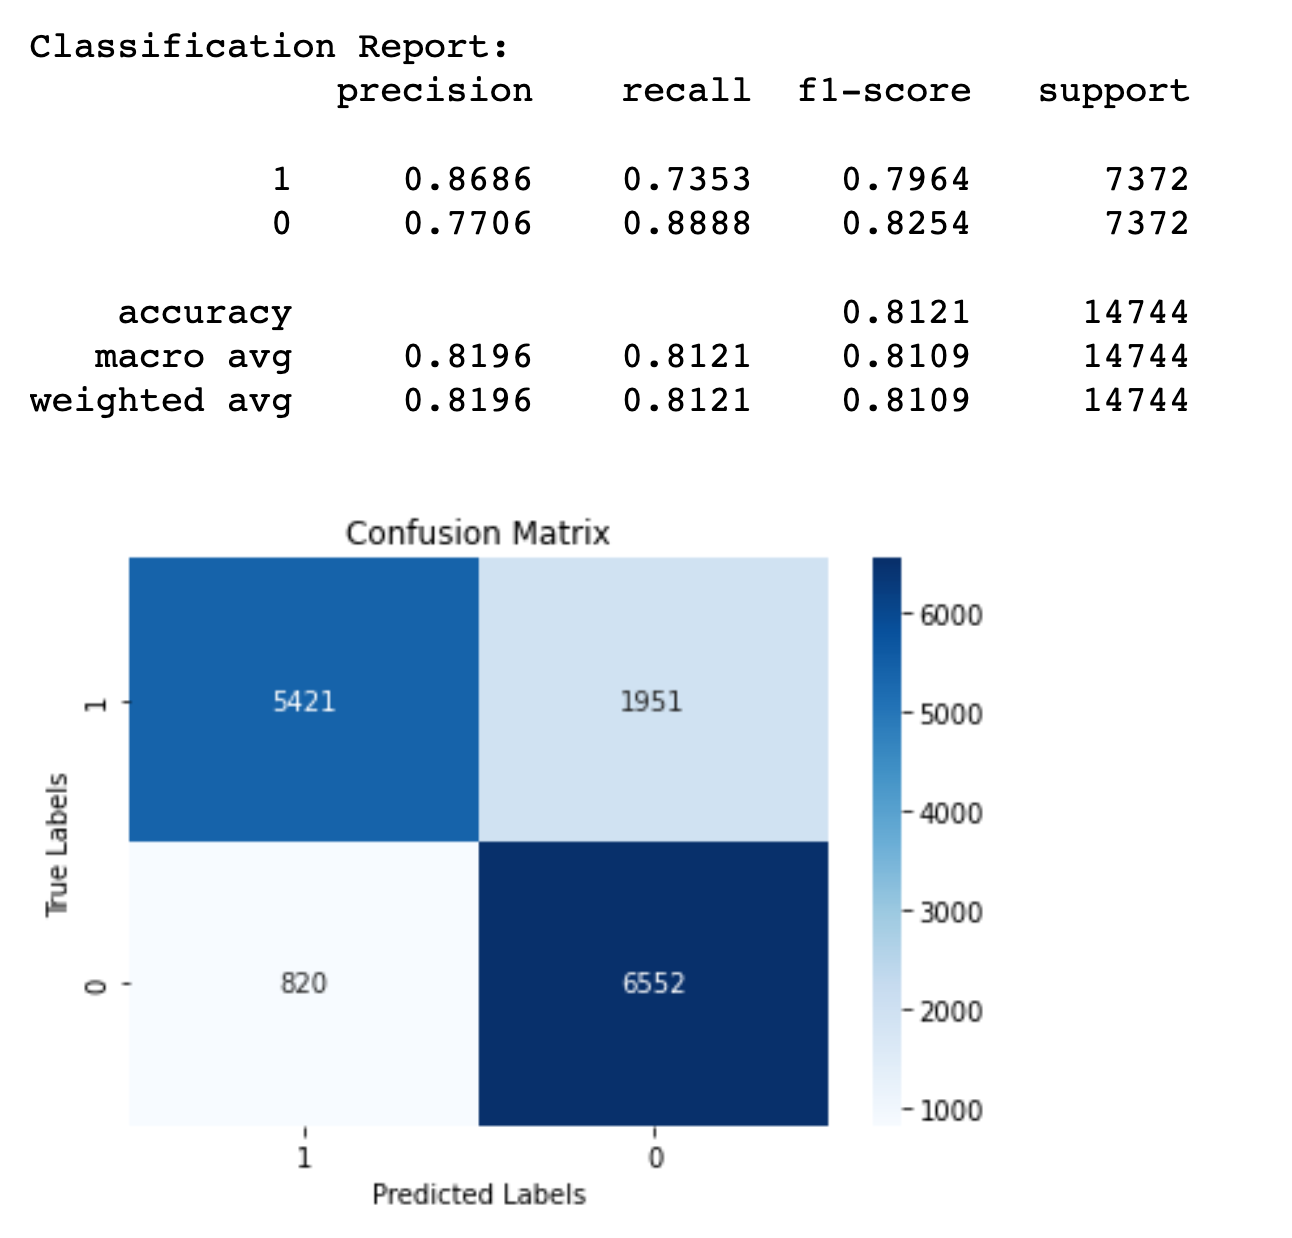
\includegraphics[scale=.6]{figures/BERT LSTM.png}
   \caption{BERT LSTM.}
   \label{fig:1}
\end{figure}


BERT TRANSFORMER
\begin{figure}[H]
    \centering
       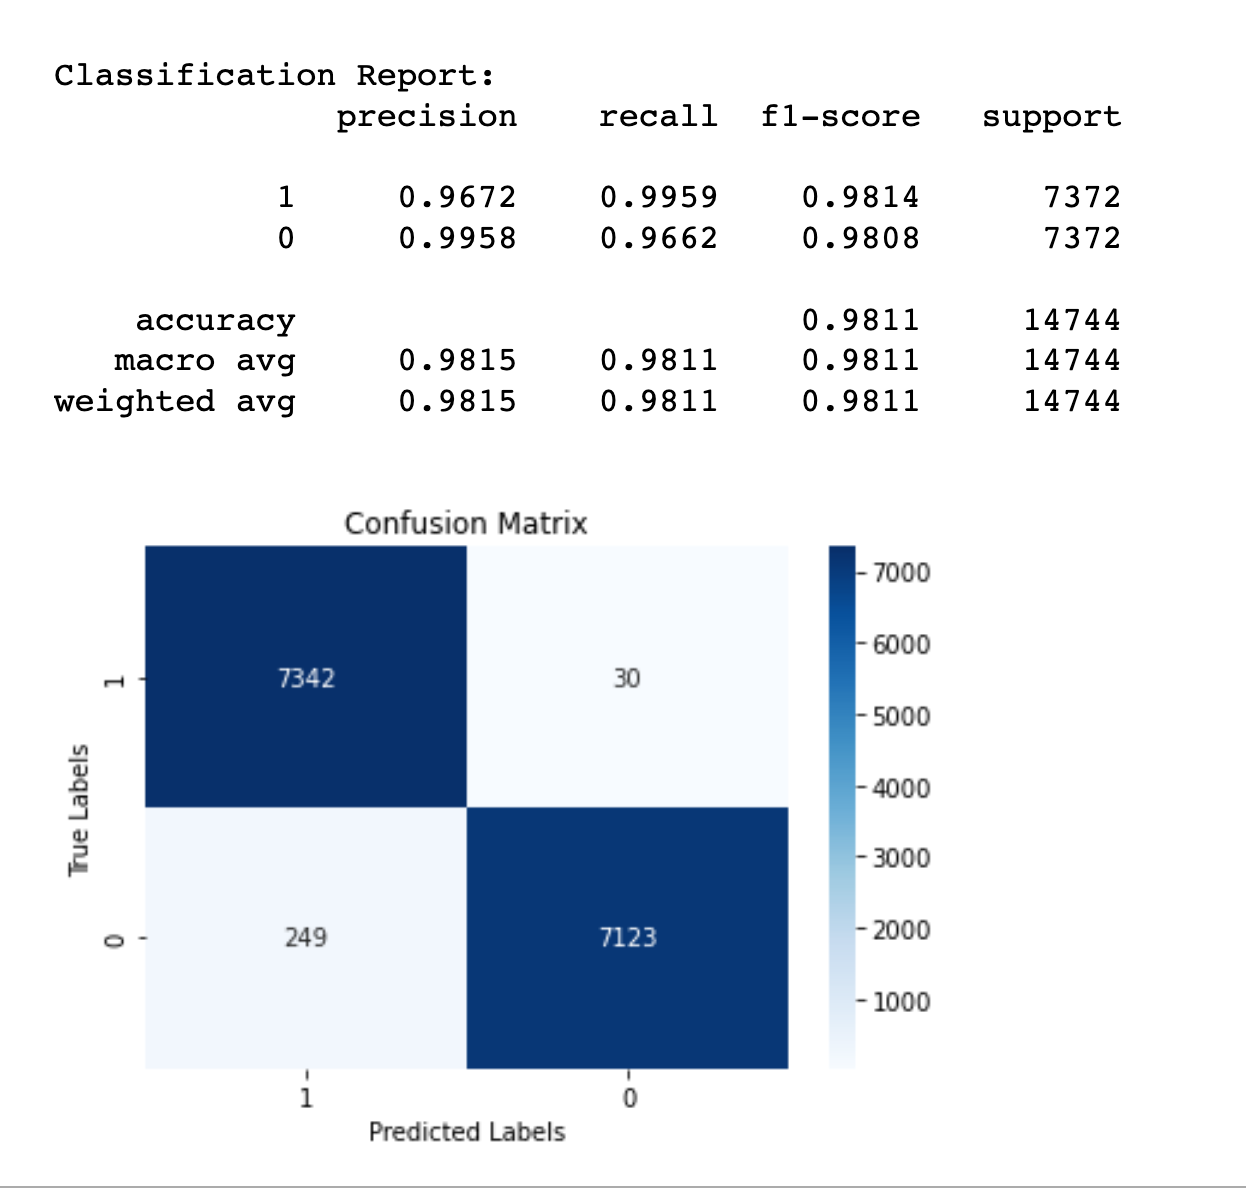
\includegraphics[scale=.6]{figures/TRANSFORMER.png}
   \caption{BERT TRANSFOMER.}
   \label{fig:2}
\end{figure}


BERT GPT-2
\begin{figure}[H]
    \centering
       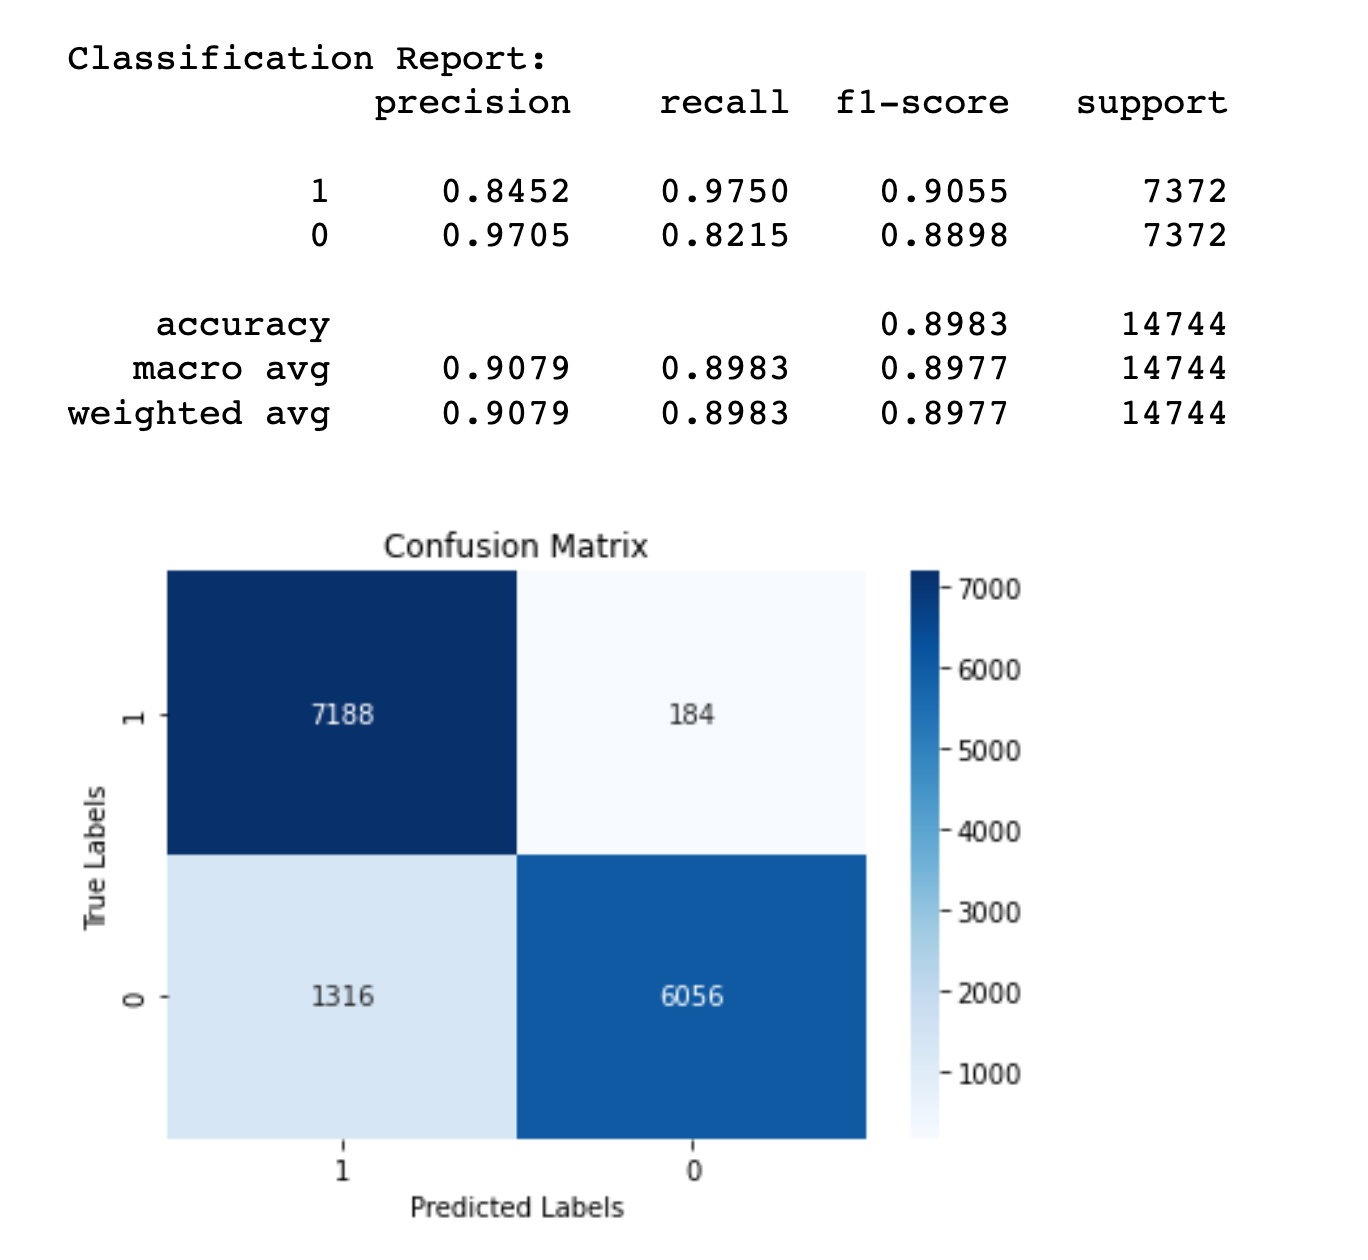
\includegraphics[scale=.6]{figures/BERT GPT.png}
   \caption{BERT GPT-2.}
   \label{fig:3}
\end{figure}

BERT LSTM + TRASNFORMER + GPT-2
\begin{figure}[H]
    \centering
       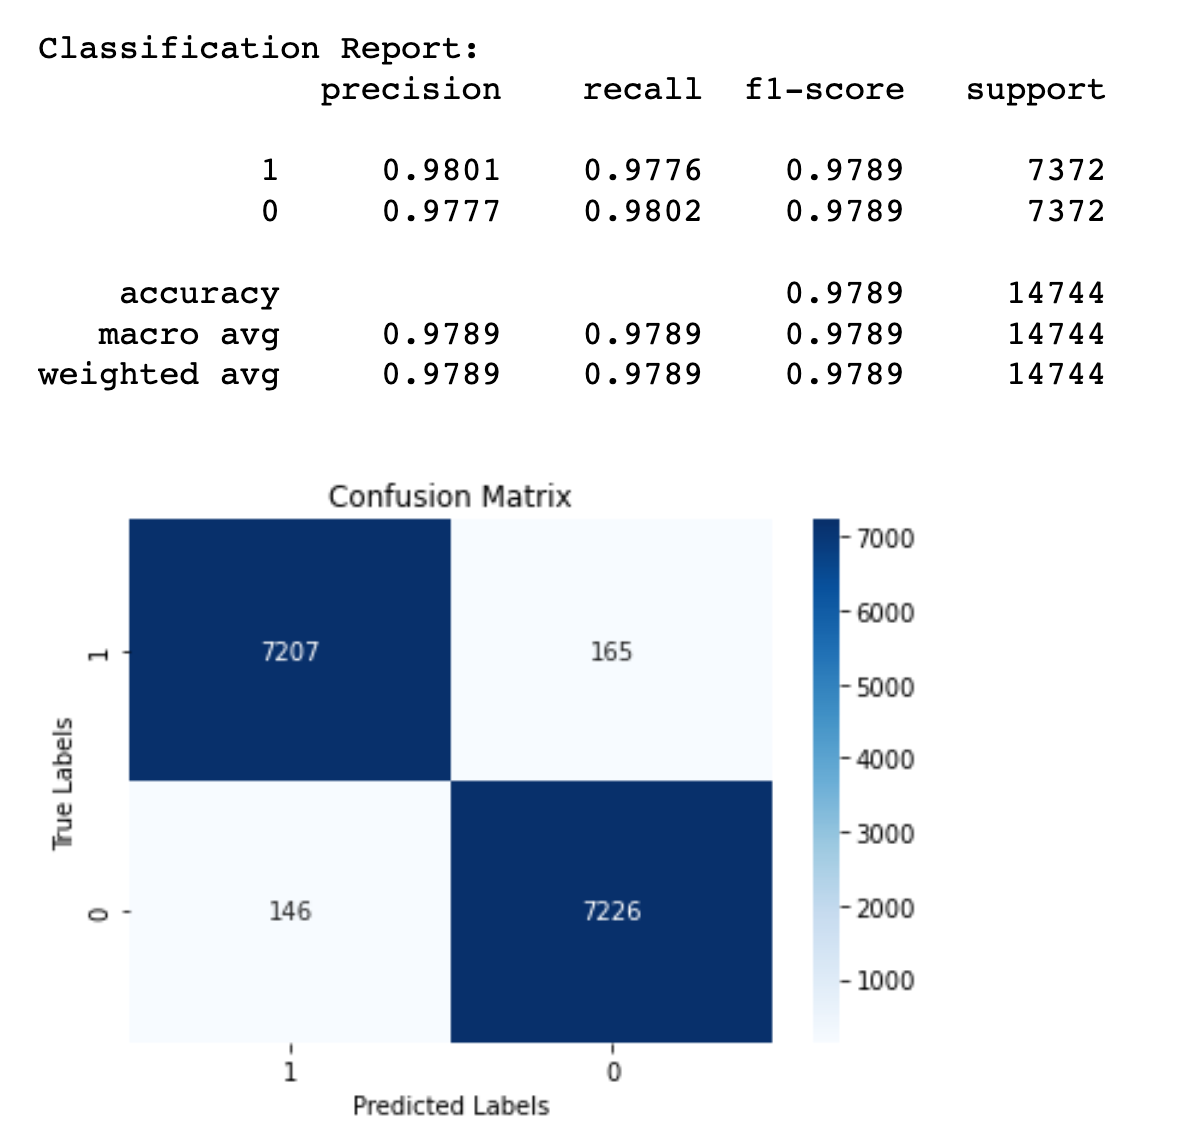
\includegraphics[scale=.6]{figures/LSTM+GPT+TRANSFORMER.png}
   \caption{BERT LSTM+GPT+TRANSFORMER.}
   \label{fig:4}
\end{figure}


BERT LSTM test SC-LSTM
\begin{figure}[H]
    \centering
       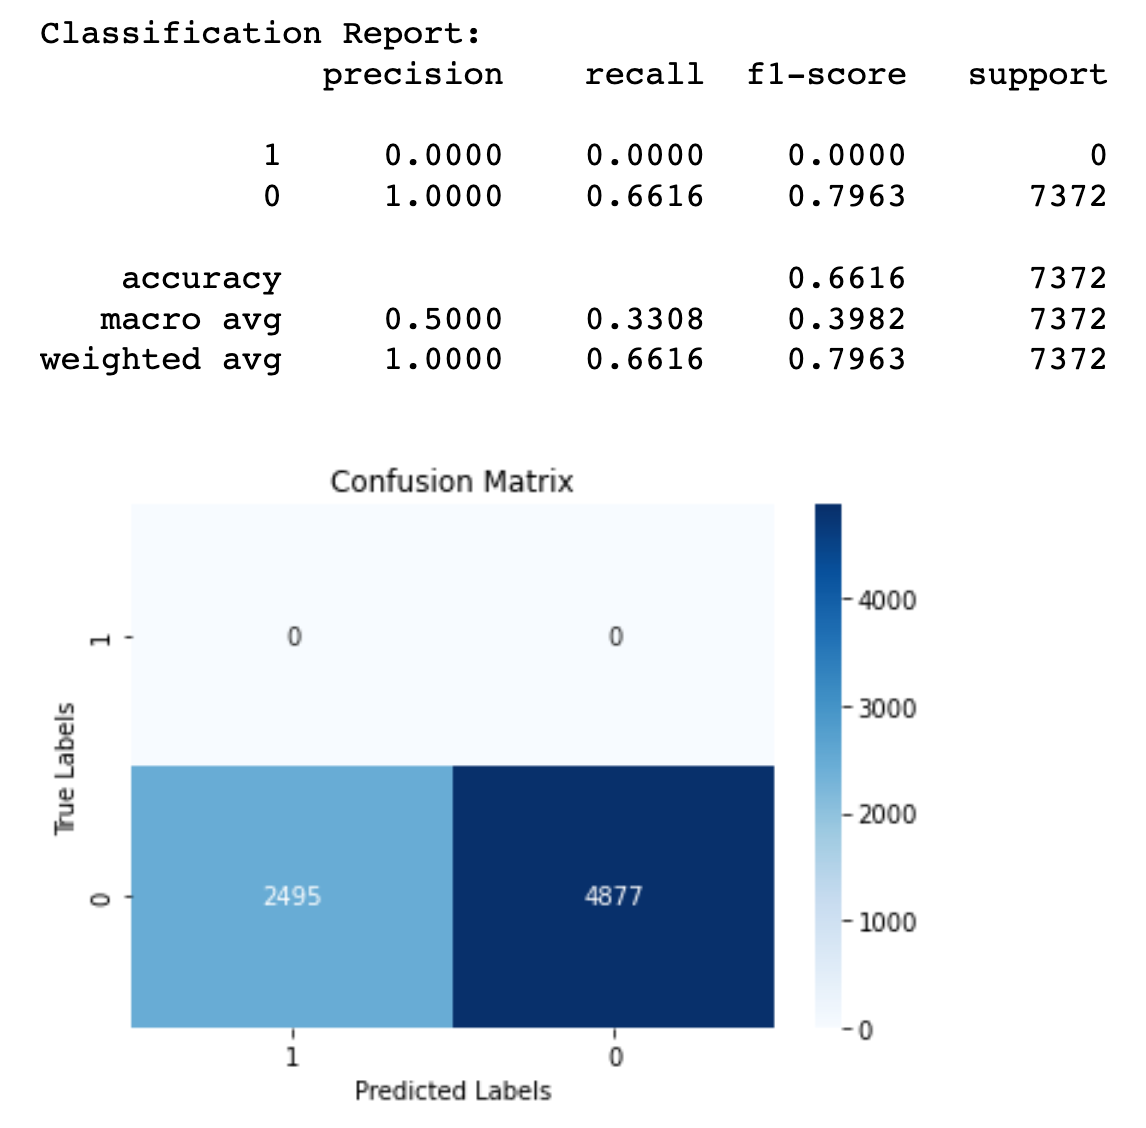
\includegraphics[scale=.6]{figures/SC-LSTM in LSTM BERT.png}
   \caption{BERT LSTM test SC-LSTM.}
   \label{fig:5}
\end{figure}
\newpage
\bibliography{references.bib} 

BERT TRANSFORMER test HDSA
\begin{figure}[H]
    \centering
       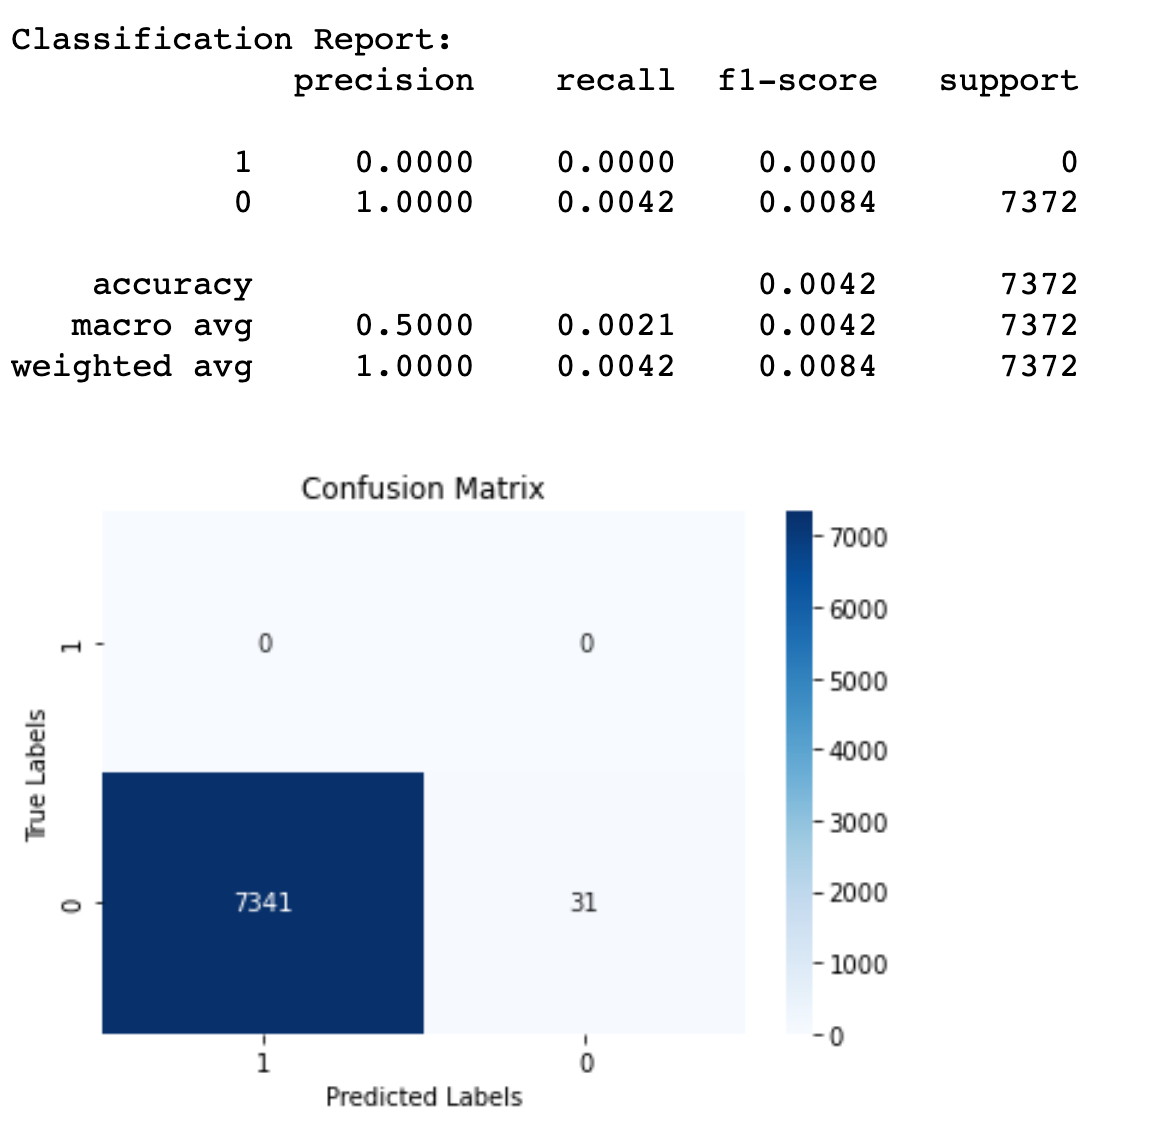
\includegraphics[scale=.6]{figures/HDSA in TRANSFOMERS.png}
   \caption{BERT TRANSFORMER test HDSA.}
   \label{fig:5}
\end{figure}
\newpage
\bibliography{references.bib} 

BERT GPT-2 test SC-GPT
\begin{figure}[H]
    \centering
       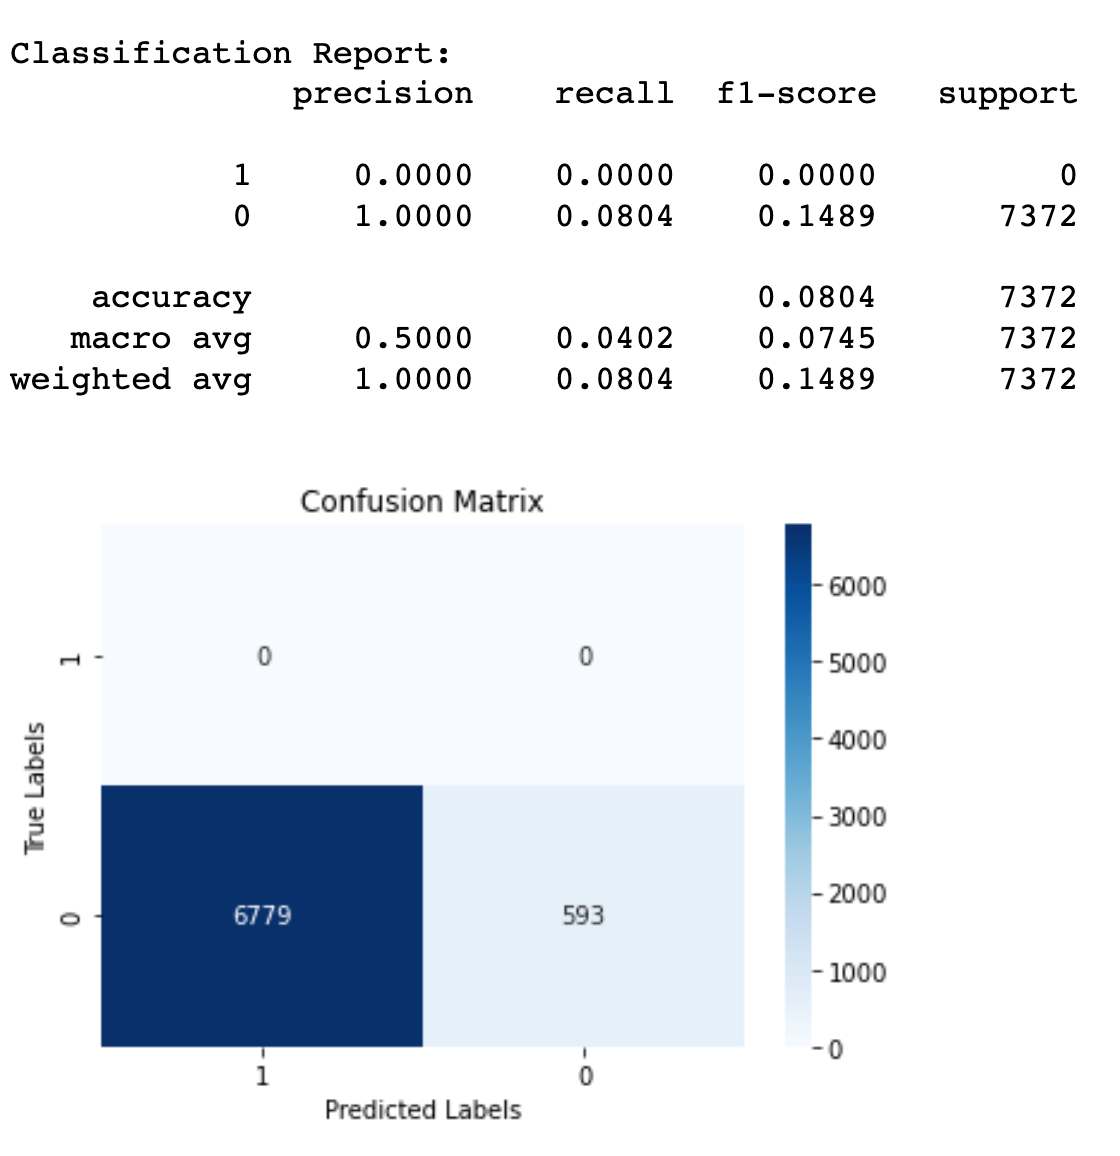
\includegraphics[scale=.6]{figures/SC-GPT in GPT BERT.png}
   \caption{BERT SC-GPT in GPT BERT.}
   \label{fig:5}
\end{figure}
\newpage
\bibliography{references.bib} 

\newpage


% %%%%%%%%%%%%%%%%%%%%%%%%%%%%%%%%%%%%%%%%%%%%%%%%%%%%%%%%%%
% %%%%%%%%%%%%%%%%%%%%%%%%%%%%%%%%%%%%%%%%%%%%%%%%%%%%%%%%%%
% FIGURES
% %%%%%%%%%%%%%%%%%%%%%%%%%%%%%%%%%%%%%%%%%%%%%%%%%%%%%%%%%%
% %%%%%%%%%%%%%%%%%%%%%%%%%%%%%%%%%%%%%%%%%%%%%%%%%%%%%%%%%%

%\begin{figure}[H]
%    \centering
 %       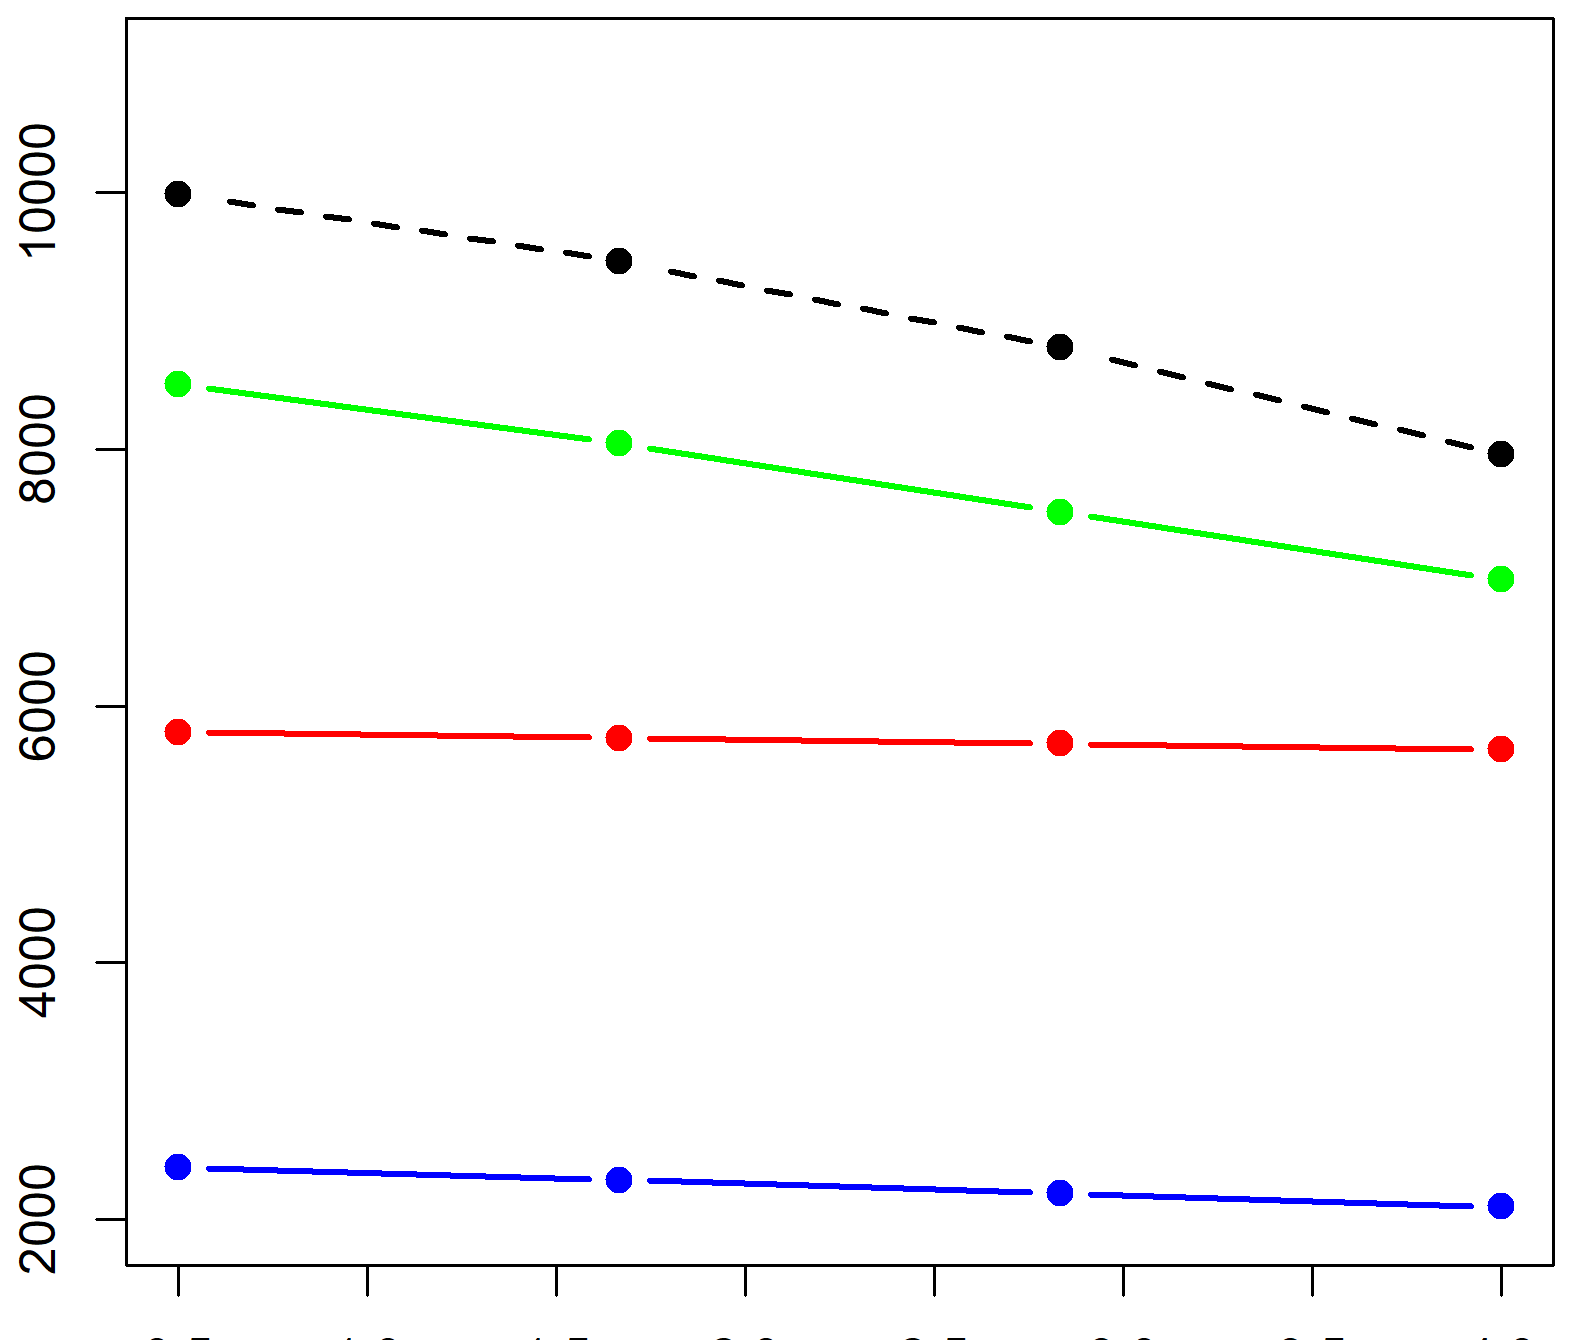
\includegraphics[scale=.6]{figures/example_figure.png}
 %   \caption{Example figure.}
 %   \label{fig:1}
%\end{figure}

% ==========================
% ==========================
% ==========================


\end{document}